\chapter{The LHCb experiment} 
\label{ch:detector}
\minitoc
 


\section{CERN and the LHC}


In the aftermath of the Second World War a number of eminent scientists proposed the creation of a collaborative European laboratory dedicated to the study of atomic physics. With this the `Conseil Europ\'een pour la Recherche Nucl\'eaire' was born; a provisional council set up in 1952 to oversee the laboratory's creation.  In 1954 the organisation as it is today was established, named the `Organisation Europ\'eenne pour la Recherche Nucl\'eaire', although the acronym CERN remained. 
The purpose of CERN was clear; the convention dictates that the organisation \emph{`shall provide for collaboration among European States in nuclear research of a pure scientific and fundamental character'}.
As such 

Furthermore, the convention stipulates that the organisation \emph{`shall have no concern with work for military requirements'} and  
requires \emph{`the results of its experimental and theoretical work shall be published or otherwise made generally available'}. 
The choice of the laboratories location followed a similar set of values, picking Geneva in Switzerland owing both to the central European location and neutrality of the host state. 


Perhaps the most well known accelerator in the complex [cite something], CERN is home to the Large Hadron Collider (LHC). Two beams of hadrons circulate in opposite directions around 27\km rings, colliding at four interaction points. The beam pipes and experimental halls are buried deep underground, providing shielding from radiation and reducing the cost of acquiring large areas of land. The tunnels traverse the Franco-Swiss border at a depth that varies between 50--175\m at the lowest and highest points respectively.      


{\color{Red}
\begin{itemize}
\item Founding of CERN and a little history 
\item Mission statement
\item Notable results and and contributions to society
\item Mention experiments other than those attached to accelerator complex
\item Time line
\item running periods? and future plans...
\end{itemize}
}

\subsection{The accelerator complex}

The LHC is only one of a vast collection of accelerators at CERN, albeit the largest. The hadrons collided in the LHC travel sequentially through a number of different machines, boosting their momentum in each. The full complex is shown in Fig.~\ref{fig:Dec_LHCb_Schematic} along with a legend detailing the types of particles considered. The protons begin life in a hydrogen gas canister. The gas is ionised and accelerated in  a linear accelerator, LINAC 2, to an energy of 50\mev. These then pass into the Proton Synchrotron Booster, raising the energy further from 50\mev to 1.4\gev. 
%%%%%%%%%%%%%%%%%%%%%%%%%%%%%%%%%%%%%%%%%%%%%%%%%%%%%%%%%%
\begin{figure}[!h]
    \centering
    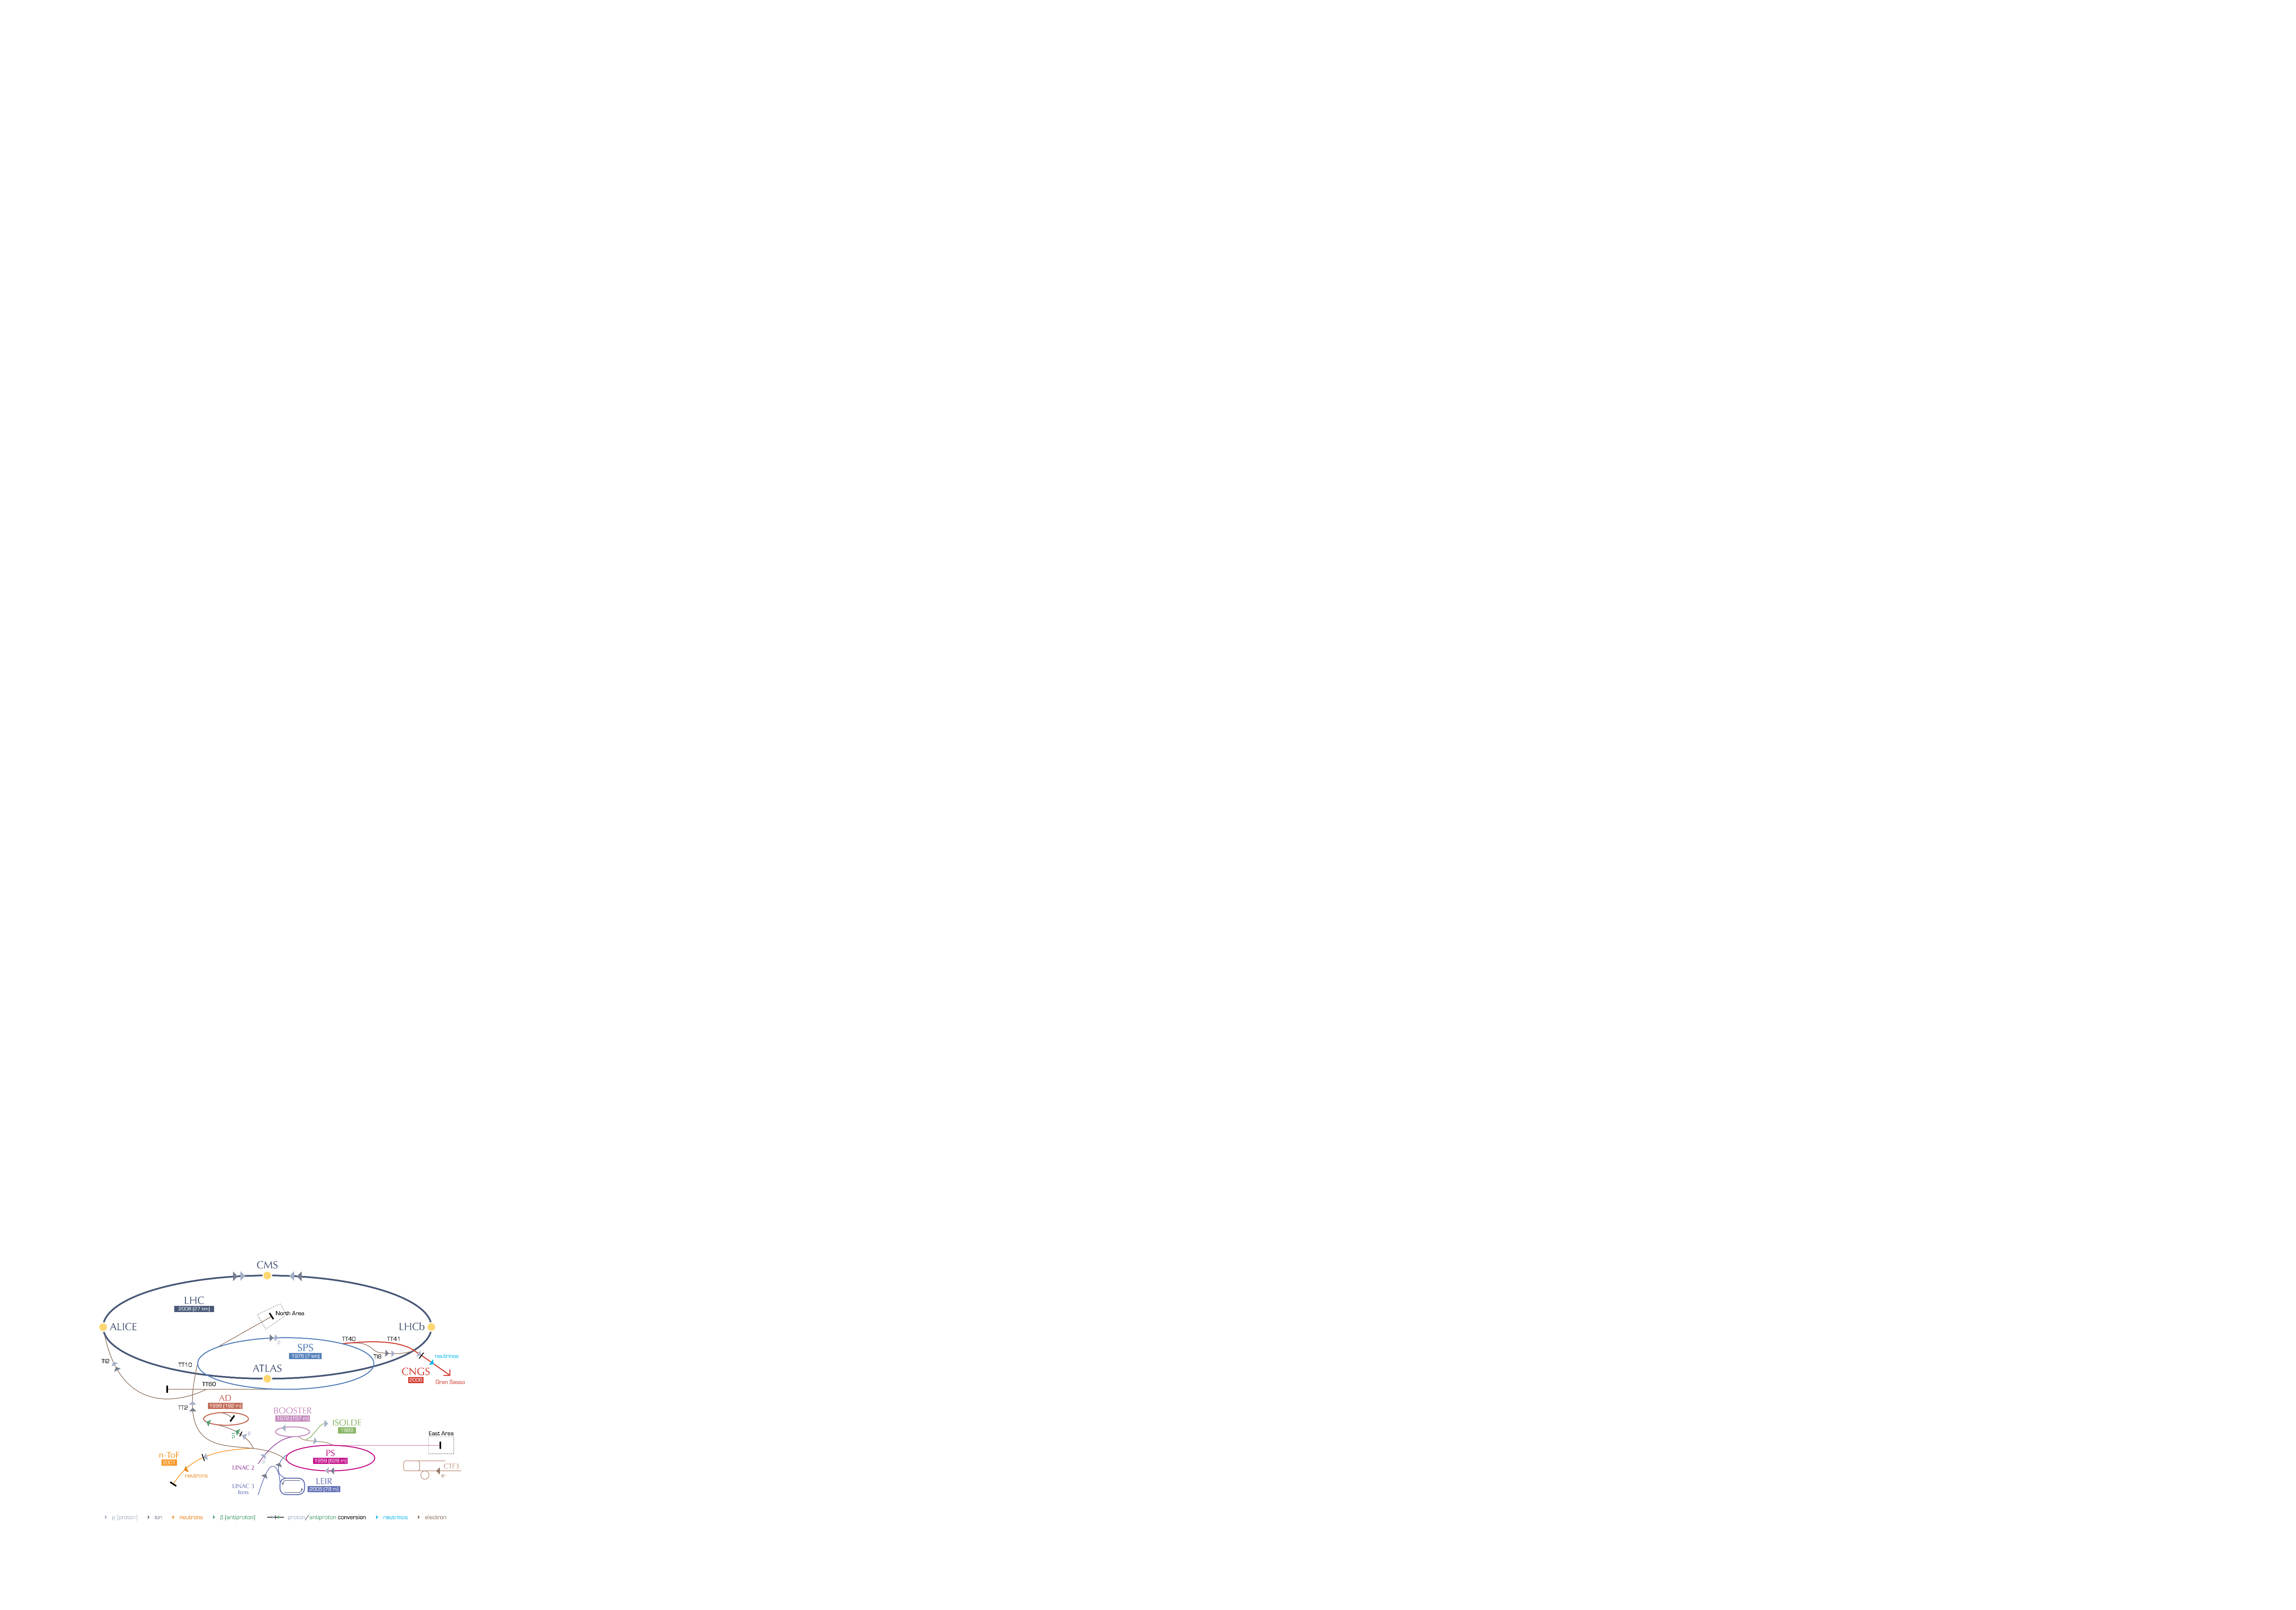
\includegraphics[width=1.0\textwidth]{figs/Detector/Acc_complex.pdf}
    \caption{The accelerator complex at CERN taken from Ref...}
    \label{fig:Dec_Acc_Complex}   
\end{figure}
%%%%%%%%%%%%%%%%%%%%%%%%%%%%%%%%%%%%%%%%%%%%%%%%%%%%%%%%%%



{\color{Red}
\begin{itemize}
\item Brief overview of the life of a proton from source to LHC
\end{itemize}
}
{\color{Green}
\begin{itemize}
\item Classic schematic of loops
\end{itemize}
}


\subsection{The LHCb collaboration} 
{\color{Red}
\begin{itemize}
\item People and counties 
\item physics aims?
\end{itemize}
}
\subsection{Beam conditions at LHCb}
{\color{Red}
\begin{itemize}
\item LHC optics
\item crossing angle
\item Luminosity levelling
\end{itemize}
}


\section{The LHCb detector}

This section provides an overview of the experimental apparatus used to obtain the data analysed in this thesis.
The \lhcb detector is comprised of distinct sub-detectors, each with a dedicated purpose. These help to characterise the sub-atomic particles created in the proton-proton collisions, and enable measurements of their kinematics, trajectories and species.
This overview includes a description of the sub-detector's construction, components and performance. 



%%%%%%%%%%%%%%%%%%%%%%%%%%%%%%%%%%%%%%%%%%%%%%%%%%%%%%%%%%
\begin{figure}[!h]
    \centering
    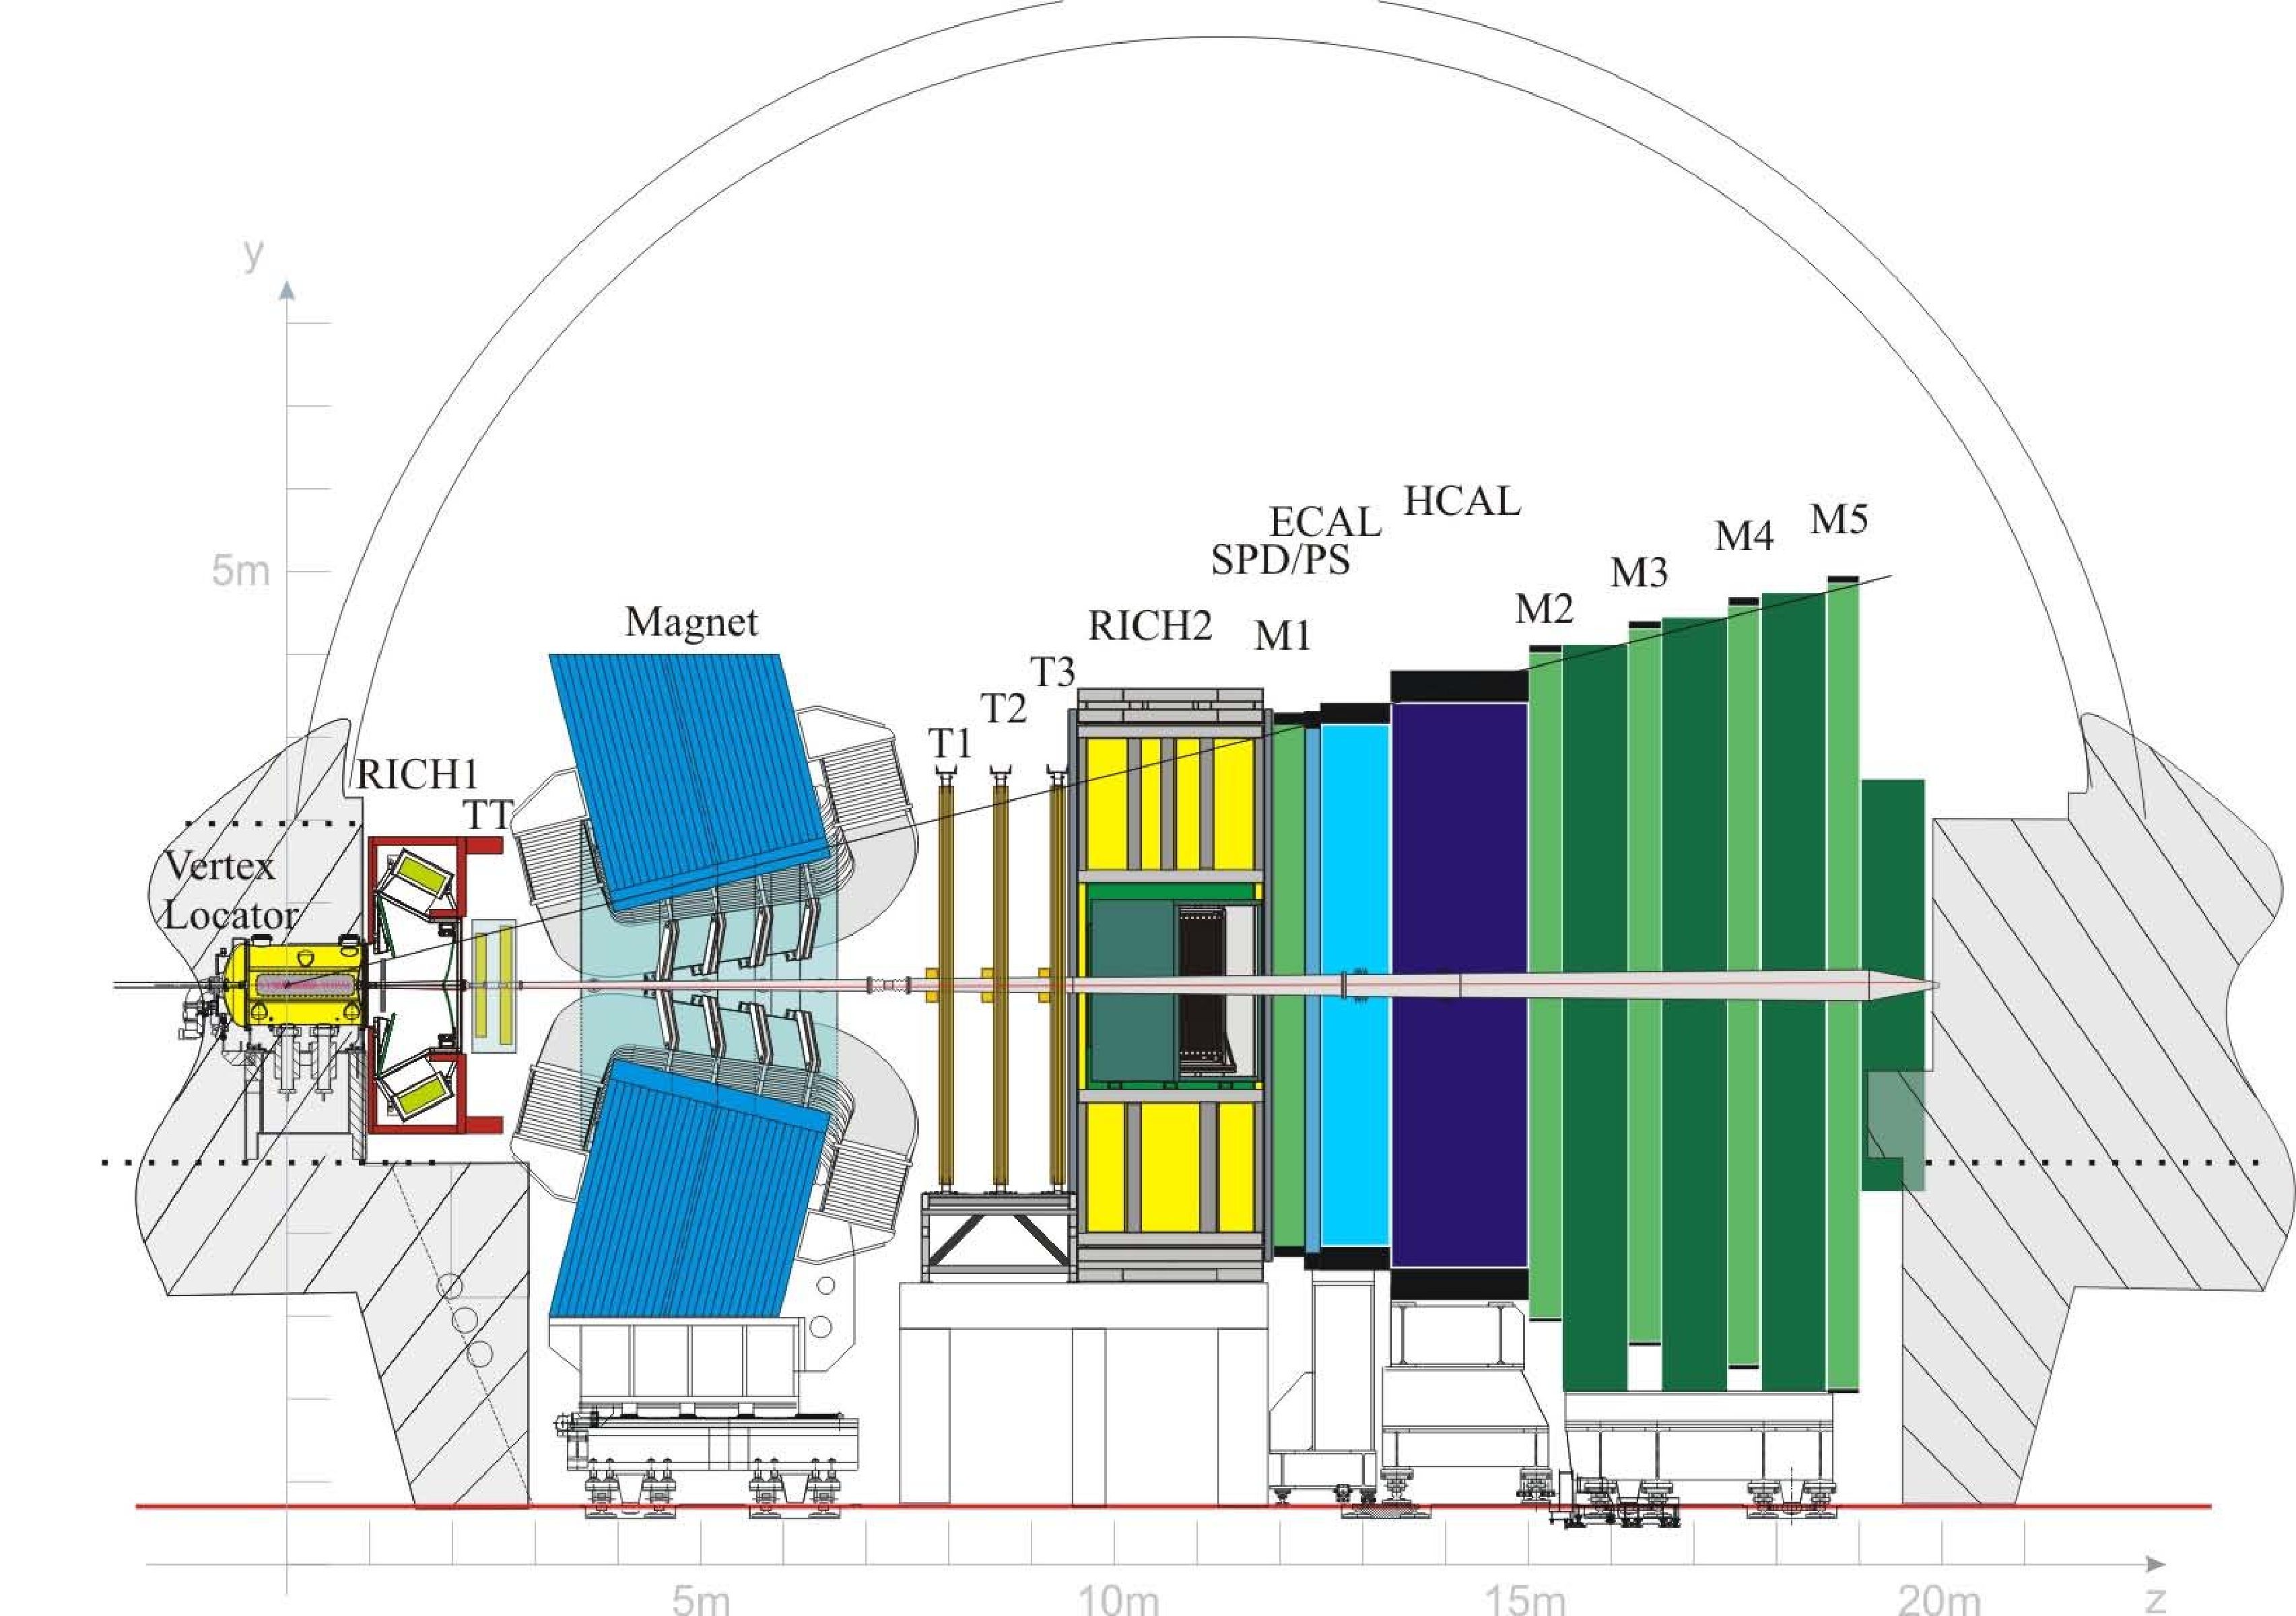
\includegraphics[width=0.8\textwidth]{figs/Detector/LHCb_Detector_Schematic.pdf}
    \caption{Schematic of the \lhcb detector from Ref.~\cite{Alves:2008zz}.}
    \label{fig:Dec_LHCb_Schematic}   
\end{figure}
%%%%%%%%%%%%%%%%%%%%%%%%%%%%%%%%%%%%%%%%%%%%%%%%%%%%%%%%%%



{\color{Red}
\begin{itemize}
\item Cavern
\item Beam pipe
\item Define axes 
\end{itemize}
}

{\color{Green}
\begin{itemize}
\item Schematic of LHCb
\item Distribution of bb pairs
\end{itemize}
}

\subsection{Magnet}

The \lhcb detector contains a warm dipole magnet that bends the trajectories of charges particles, allowing measurements of the particle's momentum. 
{\color{Red}
\begin{itemize}
\item Magnet: purpose and design 
\end{itemize}
}


\subsection{Vertex Locator}
\subsection{Silicon Tracker}
\subsection{Outer Tracker}
\subsection{Ring imaging Cherenkov detectors}
\subsubsection{\richone}
\subsubsection{\richtwo}
\subsection{Calorimeters}
\subsubsection{Pre-shower detector}
\subsubsection{Electronic Calorimeter}
\subsubsection{Hadron calorimeter}
\subsection{Muon system}
\subsection{Trigger}
\subsubsection{\lone}
\subsubsection{\hltone}
\subsubsection{\hlttwo}


\section{VELO resolution and luminosity determination}